\documentclass[12pt,a4paper,oneside]{scrartcl}
\binoppenalty=1000
\relpenalty=1000
\usepackage[unicode, pdftex,pdfborder=0 0 0,colorlinks, linkcolor=black]{hyperref}
\usepackage[utf8]{inputenc}
\usepackage[english,russian]{babel}
\usepackage{indentfirst}
\usepackage{misccorr}
\usepackage{graphicx}
\usepackage{hyperref}
\usepackage{amsmath}
\begin{document}

\title{Теоретическая Домашняя работа №2}
\author{Проничкин Юрий}
\maketitle

\section{Задание №1}
\subsection{a}
Найти $\partial max(0,1 - ax)$ \\
\\
Если $a > 0$: \\
\\
В точке $x_0 > \frac{1}{a}$: $$f(x_0) = 0 \Rightarrow f'(x_0) = 0 \Rightarrow \partial f(x_0) = 0$$
В точке $x_0 < \frac{1}{a}$: $$f(x_0) = 1 - ax_0 \Rightarrow f'(x_0) = -a \Rightarrow \partial f(x_0) = -a$$
В точке $x_0 = \frac{1}{a}$:
$$f(x_0) = 0 \Rightarrow \partial f(x_0) = \{z: f(x) \geq z(x - \frac{1}{a})\} $$
Если $x > \frac{1}{a}$: $$ 0 \geq z(x - \frac{1}{a}) \Rightarrow z \leq 0 $$
Если $x < \frac{1}{a}$: $$ 1 - ax \geq z(x - \frac{1}{a}) \Rightarrow z \geq a\frac{1 - ax}{ax - 1} = - a$$
Значит в $x_0 = \frac{1}{a}$ $\partial f(x_0) = [-a,0]$ \\
Если $a < 0$: \\
\\
В точке $x_0 < \frac{1}{a}$: $$f(x_0) = 0 \Rightarrow f'(x_0) = 0 \Rightarrow \partial f(x_0) = 0$$
В точке $x_0 > \frac{1}{a}$: $$f(x_)) = 1 - ax \Rightarrow f'(x_0) = -a \Rightarrow \partial f(x_0) = -a$$
В точке $x_0 = \frac{1}{a}$:
$$f(x_0) = 0 \Rightarrow \partial f(x_0) = \{z: f(x) \geq z(x - \frac{1}{a})\} $$
Если $x < \frac{1}{a}$: $$ 0 \geq z(x - \frac{1}{a}) \Rightarrow z \geq 0 $$
Если $x > \frac{1}{a}$: $$ 1 - ax \geq z(x - \frac{1}{a}) \Rightarrow z \leq a\frac{1 - ax}{ax - 1} = - a$$
Значит в $x_0 = \frac{1}{a}$ $\partial f(x_0) = [0,-a]$ \\
\\
Если $a = 0$: $$f(x) = 1 \Rightarrow \partial f(x) = 0 $$
\subsection{b}
Найти $\partial \sqrt{|x|}$ \\ \\
Если $ x_0 > 0 $:
$$f(x_0) = \sqrt{x_0} \Rightarrow f'(x_0) = \frac{1}{2\sqrt{x_0}} \Rightarrow \partial f(x_0) = \frac{1}{2\sqrt{x_0}}$$
Если $ x_0 < 0 $:
$$f(x_0) = \sqrt{-x_0} \Rightarrow f'(x_0) = \frac{-1}{2\sqrt{-x_0}} \Rightarrow \partial f(x_0) = \frac{-1}{2\sqrt{-x_0}}$$
Если $ x_0 = 0 $:
$$f(x_0) = 0 \Rightarrow \partial f(x_0) = \{z: f(x) \geq zx \} $$
$x > 0$:
$$ \frac{\sqrt{x}}{x} \geq z \Rightarrow \frac{1}{\sqrt{x}} \geq z \Rightarrow z \leq 0$$
$x < 0$:
$$ \frac{\sqrt{-x}}{x} \leq z \Rightarrow \frac{-1}{\sqrt{-x}} \leq z \Rightarrow z \geq 0$$
$x = 0$:
$$ 0 \geq z0 \Rightarrow z - \forall $$
Значит в $x_0 = 0 $ $\partial f(x_0) = 0$


\section{Задание №2}

По определению, т.к. в $x$ и $y$ существует субдиффиренциал: \\ \\ $f(x) \geq  f(\frac{x+y}{2}) + (z,x - \frac{x+y}{2})$ и $f(y) \geq  f(\frac{x+y}{2}) + (z,y - \frac{x+y}{2})$ \\ \\
Сложим:  $$f(x) + f(y) \geq 2f(\frac{x+y}{2}) + (z,\frac{x-y}{2}) + (z,\frac{y-x}{2}) = 2f(\frac{x+y}{2})$$ что и означает выпуклость.

\section{Задание №3}

По определению и т.к. $||0||_2 = 0 $:
$$\partial ||0|| = \{ z : ||x|| \geq (z,x)\} \Rightarrow 1 \geq \frac{(z,x)}{||x||||z||} ||z|| = cos(\phi)||z||$$
где $\phi$ - любой, значит $||z|| \leq 1 $ что и требовалось.

\section{Задание №4}

$ X_i $ - равномерно распределены по шару еденичного радиуса. Тогда вероятность попасть в шар радиуса r : $P(||X_i|| \leq r) = \frac{V_r}{V_1} $ - отношение объемов соответствующих шаров. Оно равно $r^d$ где d размерность пространства. Тогда вероятность ближайшего соседа из n попасть в шар радиуса r: 
 $$P(min(X_i) < r) = 1 - P(min(X_i) > r) = 1 - \prod_i P(X_i > r) = 1 - \prod_i(1 - P(X_i < r)) = 1 - (1 - r^d)^n$$
Тогда медиана т.е. $r : P(min(X_i) < r) = \frac{1}{2}$:
$$1 - (1 - r^d)^n = \frac{1}{2} \Rightarrow (1 - r^d)^n = \frac{1}{2} \Rightarrow r = \sqrt[d]{1 - \sqrt[n]{\frac{1}{2}}}$$
Таким образом при фиксированном d и с ростом n ближайший сосед попадает с вероятностью 0.5 в шар меньшего радиуса т.е. будет все ближе к 0, значит, если предположить что в какой-то окрестности нуля лежат объекты одного класса то при достаточно большой выборке 0 будет правильно классифицирован методом одного ближайшего соседа.
\\ 
Также с ростом d - размерности пространства медиана растет при фиксированном n т.е. в пространствах большей размерности нужно будет больше выборки для правильной классификации 0.

\section{Задание №5}
Расстояние между z и x после добавления признака: 
$\rho(z, x)^2 = p_x^2 + Z^2$ , где $p_x$ - расстояние между x и z до добавления признака, а Z - новая координата, распределенная равномерно на [0,1] \\ 
Расстояние между z и y после добавления признака: 
$\rho(z, y)^2 = p_y^2 + (Z - Y)^2$ , где $p_y$ - расстояние между x и y до добавления признака, а Y - новая координата, распределенная равномерно на [0,1] \\ 
Тогда искомая вероятность: $P(\rho(z, y)^2 < \rho(z, x)^2) = P(p_y^2 + (Z - Y)^2 < p_x^2 + Z^2)$
Посмотрим на кривую $p_y^2 + (Z - Y)^2 < p_x^2 + Z^2$, где Z, Y на $[0, 1] \times [0,1]$:
$$p_y^2 - p_x^2 = Z^2 - (Z - Y)^2 = 2YZ - Y^2, Z = \frac{p_y^2 - p_x^2 + Y^2}{2Y}$$ и так как $0 < z < 1 \Rightarrow \frac{p_y^2 - p_x^2 + Y^2}{2Y} < 1 \Rightarrow (Y - 1)^2 + p_y^2 - p_x^2 - 1 < 0 \Rightarrow (Y - 1)^2 < 1 - p_y^2 + p_x^2$ т.е. при $p_y^2 - p_x^2 > 1 $ таких в квадрате нет и искомая вероятность равна нулю (т.к. она равна площади над графиком гиперболы в пересечении с квадратом) $ \Rightarrow Y - 1 < \sqrt{1 - p_y^2 + p_x^2}, Y < 1 + \sqrt{1 - p_y^2 + p_x^2} $, что в принципе ничего не дает т.к. $ Y < 1$ и $Y - 1 > - \sqrt{1 - p_y^2 + p_x^2} \Rightarrow Y > 1 - \sqrt{1 - p_y^2 + p_x^2}$ , тогда площадь под графиком гиперболы будет: $$\int_{1 - \sqrt{1 - p_y^2 + p_x^2}}^1  \frac{p_y^2 - p_x^2 + Y^2}{2Y} dY = \frac{1}{2}(\frac{1}{2}(1 - (1 - \sqrt{1 - p_y^2 + p_x^2})^2) - (p_y^2 - p_x^2)ln(1 - \sqrt{1 - p_y^2 + p_x^2}))$$ а над графиком в квадрате :$$\sqrt{1 - p_y^2 + p_x^2} - \frac{1}{2}(\frac{1}{2}(1 - (1 - \sqrt{1 - p_y^2 + p_x^2})^2) - (p_y^2 - p_x^2)ln(1 - \sqrt{1 - p_y^2 + p_x^2}))$$ т.к. $\sqrt{1 - p_y^2 + p_x^2}$ площадь прямоугольника на котором интегрируем. Полученная функция строго убывает к 0 при увеличении разности квадратов расстояний $p_y^2 - p_x^2$ и не превосходит $\frac{3}{4}$ при совпадении расстояний до 1 и 2 точек, таким образом если разность квадратов расстояний между ближайшим и вторым соседом достаточно велика то введение нового признака, определенного только у второго и целевого объектов не будет влиять на ответ классификатора а при достаточно маленьком расстоянии вероятность поменять предпологаемый класс достаточно велика.


\section{Задание №7}

$ L(w) = ||Xw - y||_2^2, w_{k+1} = w_k - \alpha \nabla L(w_k), \Rightarrow L(w_{k+1}) = ||Xw_k - \alpha X \nabla L(w_k) - y||_2^2$ \\
$ \nabla L(w_k) = 2X^T(Xw_k - y) \Rightarrow L(w_{k+1}) = ||Xw_k - 2\alpha X^T(Xw_k - y) - y||_2^2 $, распишем его по $\alpha$: \\
$L(w_{k+1}) =  (Xw_k - 2\alpha X^T(Xw_k - y) - y , Xw_k - 2\alpha X^T(Xw_k - y) - y) =$ \\
$4\alpha^2 ||X^T(Xw_k - y)||_2^2 + 4\alpha [(X^T(Xw_k - y), y) - (Xw_k,X^T(Xw_k - y)) ] + C$, где С не зависит от $\alpha$, тогда это парабола у которой ветви направлены вверх, значит она имеет единственный минимум, найдем его:

$0 = L(w_{k+1})'_{\alpha} = 8\alpha ||X^T(Xw_k - y)||_2^2 + 4 [(X^T(Xw_k - y), y) - (Xw_k,X^T(Xw_k - y)) ]$, откуда $ \alpha = \frac{[(Xw_k,X^T(Xw_k - y)) - (X^T(Xw_k - y), y)]}{2 ||X^T(Xw_k - y)||_2^2} = \frac{(X^T(Xw_k - y),(Xw_k - y))}{2 ||X^T(Xw_k - y)||_2^2} $

\section{Задание №8}
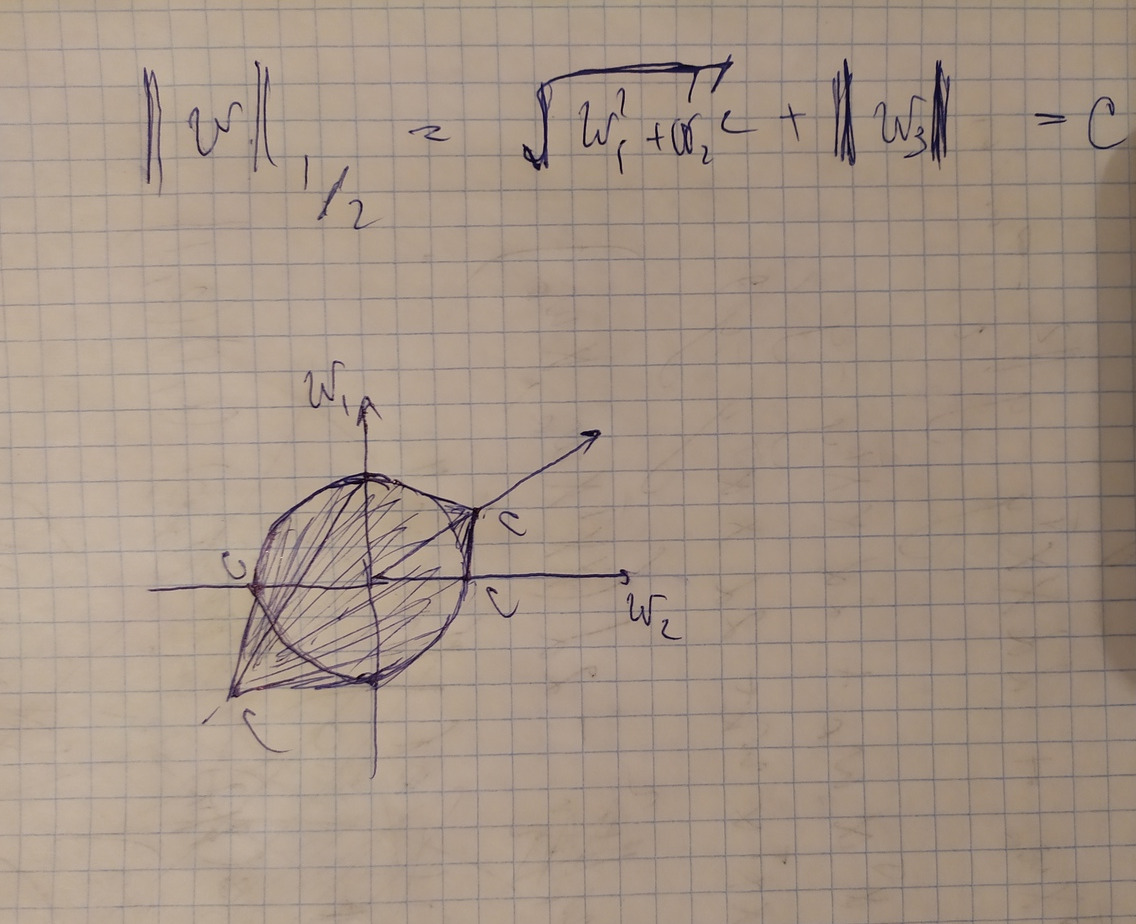
\includegraphics[scale=0.4]{Hw_pict.jpg}

Таким образом линии уровня - объеденение усеченных конусов. Таким образом если линии уровня оптимизируемой функции - концентрические окружности или элипсы, то пересечение линий уровня $||w||_{\frac{1}{2}}$ и минимальными линиями уровня оптимизируемой фукции будут пересекаться в углах графика $||w||_{\frac{1}{2}}$ (Так же как и с $l_1$ регуляризацией) , а значит это будут либо точки $|w_3| = C$ либо $\sqrt{w_1^2 + w_2^2} = C$, что и значит зануление группы признаков.
\end{document}
